\documentclass[preprint,12pt]{elsarticle}

% additional packages
\usepackage[utf8]{inputenc}
%\bibliographystyle{abbrvnat}
\usepackage{gensymb}
\usepackage{amsmath}
\usepackage{booktabs}
\usepackage{subcaption}
\usepackage{tabularx}
\usepackage{array,multirow,multicol,graphicx}
\usepackage{comment}
\graphicspath{
  {./../figures/},
}
\usepackage{lineno}
\linenumbers
% macros

\journal{Building and Environment}

\begin{document}

\begin{frontmatter}
% title
\title{Sorption Phenomena In Transient Vapor Intrusion Scenarios}

% authors
\author[Brown]{Jonathan G. V. Ström}
\author[Brown]{Shuai Xie}
\author[Brown]{Eric M. Suuberg}


\ead{eric\_suuberg@brown.edu}
\address{These authors contributed equally to this work}
\address[Brown]{Brown University, School of Engineering, Providence, RI, USA}

\begin{abstract}
Many vapor intrusion (VI) contaminants have the capacity to sorb onto a variety of materials commonly found in buildings as well as soils, yet the role and effect of sorption in VI is largely unstudied.
To bridge this gap we measure the sorptive capacities of trichloroethylene (TCE) on some materials at VI relevant concentrations; finding that material sorptive capacities vary orders of magnitudes, with cinderblock having a capacity to hold up to almost 41,000 times more contaminant than a comparable TCE contaminated air volume.
Using these experimentally derived data together with a three-dimensional numerical model of VI, we then explore the retarding effect that sorption has on contaminant transport in soils and indoor environments.
We also apply the model to investigate how the contaminant desorption from these materials, following the implementation of a successful VI mitigation scheme, affect contaminant expulsion.
We find that desorption may cause significant delay: in some cases taking months longer than if there were no sorbed contaminants.

\end{abstract}

\begin{keyword}
  Vapor intrusion \sep Temporal variability \sep Sorption \sep Attenuation factor
\end{keyword}

\end{frontmatter}

\begin{comment}

What is the message of the paper?

Sorbed contaminants can significantly delay changes in concentration in the indoor air and the soil-gas depending on the particular soil and/or indoor materials found.
This has consequences if one is for instance interested in mitigating or remediating a VI site as sorption may significantly impede this effort.
It also has consequences for rooting out indoor contaminant sources as:
1. Even after ventilation and/or removing potential indoor sources, there may still be contaminant vapors being released from various materials.
2. It may decrease the effectiveness of applying the CPM.

What is the new result/contribution that you want to describe?

This study presents some new sorption information for TCE and runs never-done-before simulations that investigate the potential role of sorption in VI and VI investigations.

What do you want to convince people of?

1. Take indoor materials into account and perhaps removing or covering up exposed materials that have a high sorption capacity.
2. Take it into consideration that contaminants vapors may emanate from soils for a long time, since they potentially have such a large sorption capacity - almost acting a source in of themselves. E.g. that remediation or mitigation effort may be impeded by this.
3. Perhaps desorbing soil/indoor material samples to determine how significant sorption might be warranted.

\end{comment}

\section{Introduction}\label{sec:intro}

% Attention grabbing intro
Most vapor intrusion (VI) contaminants have the capacity to sorb onto soil and various common indoor materials, but the role and more importantly, the consequences of these sorption processes in VI are poorly understood\cite{meininghaus_diffusion_2000,meininghaus_diffusion_2002,tillman_review_2005}.
The migration of contaminant vapors from their source into the VI impacted building and potential indoor sources is usually the prime concern in VI investigations.
Rarely are the sorbed contaminant vapors in the soil or indoor considered in an investigation.
These may potentially act as a capacitance, storing and releasing contaminant vapors in response to a change in contaminant concentration.
Consequently, contaminant vapors may be more persistent than expected at a site that has undergone remediation, potentially reducing the effectiveness of mitigation in the short term, or leading to misleading results regarding mitigation efficacy.\par

It is well recognized that building materials have the capacity to sorb pollutants.
The sorptive capacity of various volatile organic compounds (VOCs) of concern in VI has been examined on a variety of building materials, such as particle density board\cite{wang_correlation_2008}, gypsum wallboard\cite{xu_determination_2012}, and plywood and carpets\cite{bodalal_method_2000}.
However, most of these studies used relative high contaminant concentrations, usually around $\mathrm{mg/m^3}$\cite{wang_correlation_2008} or even higher.
This is several orders of magnitude higher than the concentrations relevant in VI and due to the non-linear nature of sorption with respect to concentration, sorption studies at lower concentration are needed.\par

Many VOC sorption studies have also focused on the interaction between building materials and formaldehyde\cite{xu_determination_2012}, toluene, and decane\cite{bodalal_method_2000}.
However, one of the contaminants of greatest concern in VI - trichloroethylene (TCE), has not received attention.
This is despite the fact that sorption of TCE (and other comparable VOCs) on activated carbon is extensively used to treat indoor air contamination and their sorption on passive tube samplers is widely employed for analysis of these compounds\cite{u.s._environmental_protection_agency_oswer_2015}.\par

% Some elaboration on these consequences? E.g. cover:
% - EPA site investigation recommendations
% - CPM and potential issues
% - Remediation (are there any examples of vapor being more persistent?)
% Separate paragraph for each?

Over the years many VI sites have been investigated.
Two well-known examples of these are the studies of a house in Layton, Utah and one in Indianapolis, Indiana.
Both of these sites were outfitted with a wide variety of instrumentation to measure various metrics such as contaminant concentration in interior, soil, and groundwater, as well as pressure, temperature, or weather.
These studies yielded some of the richest VI datasets available and gave invaluable insights into the VI process, including into the application of CPM\cite{holton_long-term_2015} and sub-slab depressurization (SSD) mitigation systems\cite{lutes_comparing_2015,u.s._environmental_protection_agency_assessment_2015}.
However, neither of these studies considered the role that sorption may have had at these sites.\par

The potential impact of sorption could perhaps be most significant in situations in which contaminant entry rates vary widely with time, such as in the application of the controlled pressure method (CPM) and various mitigation schemes.
The controlled pressure method involves the forced over- and depressurization of a building to maximize or minimize the contaminant entry rate into the building.
This can help the investigator ascertain the worst-case VI scenario and help identify potential indoor contaminant sources\cite{mchugh_recent_2017,holton_long-term_2015}.
However, if the building indoor materials have a large sorptive capacities, then desorption and sorption processes may significantly affect the indoor air contaminant concentration.
Likewise, a significant amount of sorbed contaminant may be released from interior materials over an unknown period of time after mitigating the contaminant intrusion at a site\cite{meininghaus_diffusion_2000,meininghaus_diffusion_2002}.\par

% Why use modeling for this? Cover:
% - Briefly why we wish to model
% - Sorption in other models and their applications (or lack thereof I should say)
In the past, VI models have been used to gain further insight into VI processes. % TODO: Add some citations here.
Previous examples of VI modeling studies include one on the role of rainfall in VI\cite{shen_numerical_2012}, or drivers of temporal variability in some of the aforementioned sites\cite{strom_factors_2019}.
However, while many VI models are presented including a sorption term in the governing equation for contaminant transport in soils, none have really explored the role of sorption in VI in a transient simulation.
The reason for this is two-fold.
First, there has been a general lack of interest in sorption related to VI thus far.
Secondly, the vast majority of VI modeling efforts and studies have focused on steady-state analyses of VI, and sorption only affects soil contaminant transport in time-dependent scenarios.\par

% Final paragraph - outlining what we will do:
To bridge this knowledge gap we will explore the role of sorption in VI by considering the signifnance of newly obtained contaminant sorption data in the context of VI models.
Sorption data of TCE on various materials, including cinderblock, drywall, wood, paper, carpet, and Appling soil have been measured in a fixed bed sorption experiment.
These sorption data are used to generate sorption parameters to be used in a three-dimensional finite element VI model.
For this purpose we will consider a prototypical VI scenario where a free-standing house, with a basement, is overlying a homogenously contaminated groundwater source.
Using this model we investigate how contaminant transport is affected by sorption, how indoor sorptive materials affect indoor air concentration as the building's pressurization fluctuates and how indoor air concentration are affected by indoor materials following successful mitigation of the structure.\par

\section{Methods}\label{sec:methods}

\subsection{Experimental Setup}\label{sec:experimental_method}

The TCE  dynamic sorption process of different building materials were determined by use of a method schematically shown in Figure \ref{fig:js_sx_setup}.
This method involved a selected material contained in an adsorption column through which TCE-containing gas was passed, and subsequent thermal desorption and measurement of the total amount of adsorption.
During the adsorption part of the process, stainless steel tubes were packed with building materials held in place by glass wool.
The amount of building material normally held in the tube was around 1 g. % TODO: (I forget which materials we used in this manuscript. drywall=2 g, leather=2 g).
It was determined that neither the glass wool nor the stainless steel tube would retain significant amounts of TCE.
The sample-containing tubes were first exposed desired low concentrations of TCE in nitrogen, which were then allowed to interact with the flow for varying periods of time.
The typical flow rate of the nitrogen was 60 ml/min and the concentrations of TCE was around 1.1 ppbv.
All of these adsorption experiments were conducted at room temperature.
After a given time of exposure to the TCE-containing flow, that flow was stopped, and the sample tube was attached to a sorbent tube placed downstream of the sample tube.
The sample tube was arranged such that the direction of the nitrogen flow in the subsequent desorption process was opposite that of the TCE-containing nitrogen flow during the adsorption process.
During the thermal desorption step, the sample containing tube was covered by a heating mantle which permitted its heating at 100 \degree C.
This allowed fully desorbing the TCE which had been held on the sample into a pure nitrogen flow, which carried it to the room temperature downstream sorbent tube, where it was again fully adsorbed.
These tubes fully capture all of the TCE desorbed, from the samples, and the amount of TCE was analyzed by Gas Chromatography (GC) with an  Electron Capture Detector(ECD).

\begin{figure}
  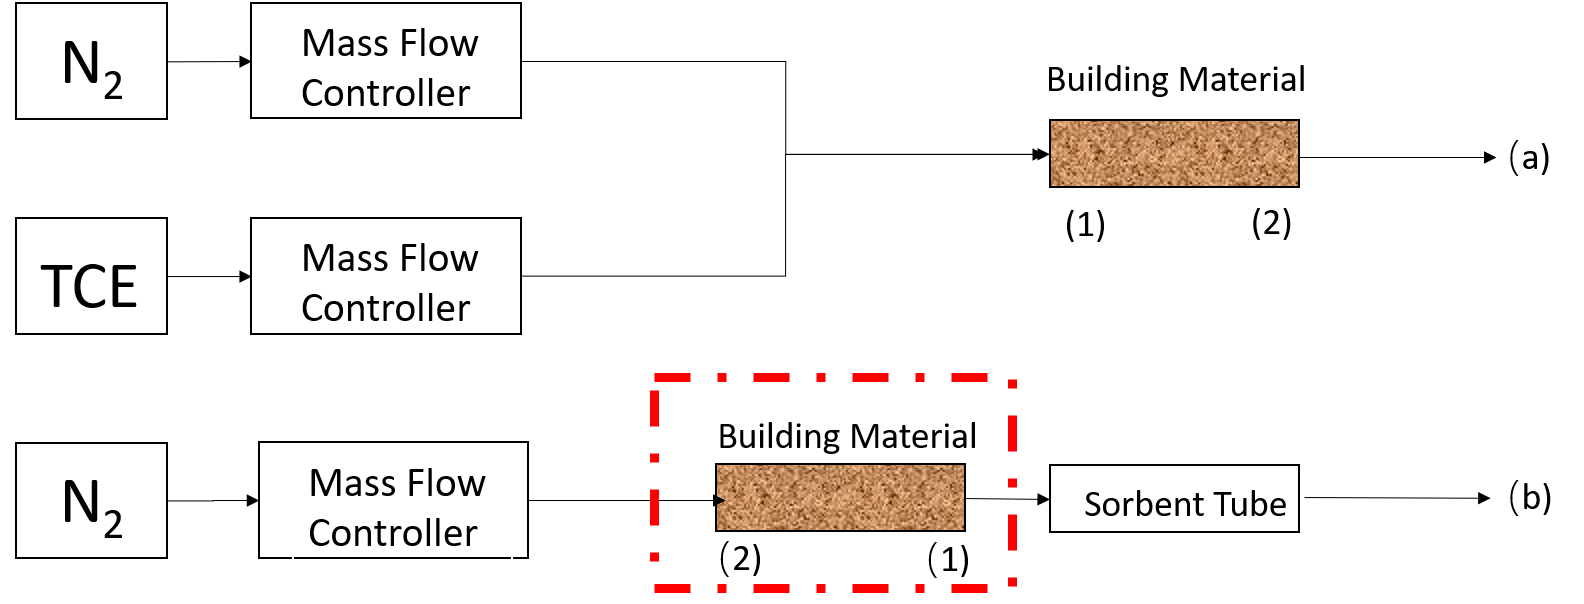
\includegraphics[width=\textwidth]{JS_SX_experiment_setup.png}
  \caption{Schematic of experimental setup.} % TODO: Shuai: Write better description
  \label{fig:js_sx_setup}
\end{figure}

% TODO: Add a mention/reference to how the experimental data is then used to get kinetic data further down.

\subsection{Numerical Model}\label{sec:model}

To investigate the role of sorption in VI, we consider a simple VI scenario.
Here we consider a house with a 10 by 10 m footprint, with the foundation bottom located 1 m below ground surface (bgs).
The sole contaminant source is an uniformly TCE contaminated groundwater located 4 bgs, and the soil surrounding the house is assumed to homogenous and of a singular type.
All contaminant vapors are assumed to enter the house through breaches in the foundation, modeled as a 1 cm wide crack that runs along the perimeter of the house.
Finally we assume that sorption processes can occur both in the soil matrix and in the indoor environment (on various indoor materials).\par

Modeling this scenario requires us to simulate a couple of physics, many of which depend and interact with each other.
The governing equations and the physics they govern are:
\begin{enumerate}
  \item van Genuchten retention model - soil moisture.
  \item Darcy's Law - air flow in the porous media.
  \item Transport equation - contaminant transport in porous media.
  \item Continuously stirred tank reactor (CSTR) - contaminant concentration in the indoor environment.
\end{enumerate}
These physics are implemented in COMSOL Multiphysics, a commercial finite-element method package, which is used to solve our model.
It is important to note that the indoor environment is implicitly modeled, but instead only given by the CSTR equation; the soil domain is explicitly modeled.\par

% TODO: Make some nice figure
\begin{figure}
  %\includegraphics{}
  \caption{The vapor intrusion model}
  \label{fig:model}
\end{figure}

\subsubsection{Vadose Zone Moisture Content}

Since the contaminant transport occurs through three-phased the vadose zone, it is important that we correctly account for soil moisture content and its effect on advective and diffusive transport.
In this modeled scenario, we assume that the soil moisture is at steady-state and does not change, and thus the soil moisture content is given by the retention model developed by van Genuchten.\par

The van Genuchten retention model gives the soil water saturation as a function of elevation above groundwater.
In turn this gives the water and gas filled porosities, and the relative permeability of the soil matrix.
\begin{align}
  % saturation
  \mathrm{Se} &=
    \begin{cases}\label{eq:van_genuchten_saturation}
      \frac{1}{(1 + \alpha z^n)^m} & z < 0 \\
    1 & z \geq 0
    \end{cases} \\
  % soil moisture
  \theta_w &=
    \begin{cases}\label{eq:van_genuchten_soil_moisture}
      \theta_r + \mathrm{Se}(\theta_s - \theta_r) & z < 0 \\
      \theta_s & z \geq 0
    \end{cases} \\
  % relative permeability
  k_r &=
    \begin{cases}\label{eq:van_genuchten_relative_permeability}
      \mathrm{Se}^l \big[ 1 - \big( 1 - \mathrm{Se}^\frac{1}{m} \big) \big]^2 & z < 0 \\
      0 & z \geq 0
    \end{cases}
\end{align}
$\mathrm{Se}$ is the saturation, and ranges from 0 to 1, which represent completely un- to fully saturated;
$z$ is the elevation above the groundwater in meters;
$\theta_r$, $\theta_s$, $\theta_w$, and $\theta_g$ are the residual moisture content, saturated porosity (or just porosity), and water and air filled porosities respectively. All units are in volume of phase divided by the volume of soil;
$k_r$ is the relative permeability of water, which modifies the saturated permeability. This too ranges from 0 to 1, indicating completely im- and permeable respectively. $1-k_r$ gives the relative permeability of air.\par

\subsubsection{Gas Flow In The Vadose Zone}\label{sec:darcy}

The gas flow in the vadose zone is governed by a modified version of Darcy's Law.
Originally, Darcy's Law was developed to describe flow in saturated porous media, but since we're interested in flow in unsaturated media, modification is necessary.
An effective permeability that depends on the relative permeability from van Genuchten is introduced to allow for correct flow profiles in unsaturated porous media.\par

The vapor flow governing equation is given by
\begin{equation}\label{eq:darcy}
  \frac{\partial}{\partial t} (\rho \theta_s) + \nabla \cdot \rho \Big( -\frac{(1-k_r) \kappa}{\mu} \nabla p \Big) = 0
\end{equation}
Here $\rho$ is the fluid density;
$\nabla$ is the del operator;
$\kappa$ is the saturated permeability;
$\mu$ is the fluid viscosity; and $p$ is the fluid pressure.
We assume that the contaminant vapors are so dilute that the gas flow properties can be taken to be those of air, and specifically at 20 \degree C and all the transport properties may be found in Table \ref{tbl:model}.\par

\paragraph{Boundary Conditions}

To solve \eqref{eq:darcy} we assign the atmosphere boundary (see Figure \ref{fig:model}) to be at reference pressure and act as a gauge, i.e. zero pressure.
The foundation crack boundary is assigned the indoor-outdoor pressure difference value.
Remaining boundaries are no-flow boundary conditions.
\begin{align}
  &\text{Atmosphere} &p = 0 \; \mathrm{(Pa)} \\
  &\text{Foundation crack} &p = p_\mathrm{in/out} \; \mathrm{(Pa)} \\
  &\text{All other} &-\vec{n}\cdot\rho_\mathrm{air}\vec{u} = 0 \; \mathrm{(kg/(m^2\cdot s))}
\end{align}
Here $\vec{n}$ and $\vec{u}$ are the boundary normal and gas velocity vectors.

\paragraph{Initial Conditions}

For steady-state problems, the initial conditions don't matter, but is simply zero for the entire domain.
When solving transient, the initial conditions are given by the steady-state solution.\par

\subsubsection{Mass Transport In The Vadose Zone}\label{sec:mass_transport}

Contaminants in the vadose zone exist in three phases - gaseous, solved in water, and sorbed onto soil particles.
While there are three distinct phases, the water and gas phases are related via Henry's Law \eqref{eq:henrys_law}.
\begin{equation}\label{eq:henrys_law}
  c_g = K_H c_w
\end{equation}
Where $c_g$ and $c_w$ are the gas and water phase concentrations respectively in $\mathrm{mol/m^3}$;
$K_H$ is the dimensionless Henry's Law constant.\par

In this work, we consider sorption between the soil and vapor phases, as a function of the water contaminant concentration, through linear sorption \eqref{eq:linear_sorption}.
\begin{equation}\label{eq:linear_sorption}
  c_s = K_\mathrm{ads} \rho_b c_g = K_\mathrm{ads} \frac{\rho}{1-\theta_t} K_H c_w
\end{equation}
Here the $c_s$ is the solid phase concentration in $\mathrm{mol/kg}$;
$\rho_b$ is the bulk density of the soil $\mathrm{kg/m^3}$, which is given by the density $\rho$ and the total soil porosity $\theta_t$;
$K_\mathrm{ads}$ is the sorption isotherm in $\mathrm{m^3/kg}$.
Using Henry's Law and the linear isotherm we can express the total contaminant concentration in terms of the water contaminant concentration.\par

Mass transport in the vadose zone is governed by diffusion and advection and is given by \eqref{eq:mass_transport}.
\begin{equation}\label{eq:mass_transport}
  R \frac{\partial c}{\partial t} =
    \nabla \cdot[ D_\mathrm{eff} \nabla c] -
    K_H \vec{u} \cdot \nabla c
\end{equation}
The first term in \eqref{eq:mass_transport} gives the change in contaminant water concentration with respect to time, modified by the \textit{retardation factor}, $R$, which is discussed below;
The second is the effective diffusive flux which is modified by the effective diffusion coefficient $D_\mathrm{eff}$ which is also discussed below.
The third is the advective flux where $\vec{u}$ is the soil-gas velocity from Darcy's Law, which when multiplied with $K_H$ gives the gas phase concentration advective flux.\par

\paragraph{Contaminant entry into the building}

The contaminant enters the building through a combination of advection and diffusive fluxes and is given by \eqref{eq:contaminant_entry}.
\begin{equation}\label{eq:contaminant_entry}
  j_{ck} = \begin{cases}
    u_{ck} c_g - \frac{D_\mathrm{air}}{L_\mathrm{slab}} (c_{in} - c_g) & u_{ck} \geq 0 \\
    u_{ck} c_{in} - \frac{D_\mathrm{air}}{L_\mathrm{slab}} (c_{in} - c_g) & u_{ck} < 0
\end{cases}
\end{equation}
Here the $j_{ck}$ is the molar contaminant flux into the building in $\mathrm{mol/(m^2 \cdot s)}$;
$D_\mathrm{air}$ is the contaminant diffusion coefficient in pure air in $\mathrm{m^2/s}$;
$L_\mathrm{slab}$ is the thickness of the foundation slab in $\mathrm{m}$.
The flux expression changes if there is a bulk flow into the building, i.e. $u_{ck} \geq 0$, or out of the building.

\paragraph{Retardation factor}

As the contaminants are transported through the vadose zone, the partitioning between the various phases increases the contaminant residency time, retarding the transport of contaminants.
This effect is represented by $R$ which is the retardation factor \eqref{eq:retardation_factor}.
\begin{equation}\label{eq:retardation_factor}
  R = \theta_w + \theta_g K_H + \rho_b K_H K_\mathrm{ads}
\end{equation}
Here $\theta_w$, $\theta_g$ are the water and gas filled soil porosities;
$K_\mathrm{ads}$ is the solid-gas phase sorption isotherm in $\mathrm{m^3/kg}$.
The diffusive and advective transport retardation is proportional to the inverse of $R$.
\begin{align}
  D_\mathrm{retarded} &= \frac{D_\mathrm{eff}}{R} \\
  \vec{u}_\mathrm{retarded} &= \frac{\vec{u}}{R}
\end{align}
It should be noted that the soil-gas velocity, $\vec{u}$, is not retarded in of itself, but rather just the contaminant being transported through advection, giving a effective bulk velocity.\par

\paragraph{Effective diffusivity}

The effective diffusivity in the vadose zone varies with the soil moisture content, from being close to that in water when fully saturated and vice versa.
Millington-Quirk developed \eqref{eq:millington-quirk} which describes the effective diffusivity in variably saturated porous media.
\begin{equation}\label{eq:millington-quirk}
  D_\mathrm{eff} = D_\mathrm{water} \frac{\theta_w^\frac{7}{3}}{\theta_t^2} + \frac{D_\mathrm{air}}{K_H} \frac{\theta_g^\frac{7}{3}}{\theta_t^2}
\end{equation}
Where the porosity fractions are the water and gas phase tortuosity terms;
$D_\mathrm{air}$ and $D_\mathrm{water}$ are the contaminant diffusion coefficient in air and water respectively in $\mathrm{m^2/s}$.\par

\paragraph{Boundary Conditions}

A few boundary conditions are required to solve \eqref{eq:mass_transport}.
In this model, the sole contaminant source is assumed to be the homogenously contaminated groundwater, which we assume to have a fixed concentration.
The atmosphere acts as a contaminant sink, and any contaminant that makes it to this boundary is ifinitely diluted, thus this is simply a zero concentration boundary condition.
Contaminants leave the soil domain and enter the building through a combination of advective and diffusive gas phase transport.
The last boundary condition is applied to all other boundaries and is a no-flow boundary.
\begin{align}
  &\text{Groundwater} & c_w = 0 \; \mathrm{(mol/m^3)} \\
  &\text{Atmosphere} & c_w = c_{gw} \; \mathrm{(mol/m^3)} \\
  &\text{Foundation crack} & -\vec{n} \cdot \vec{N} = - \frac{j_{ck}}{K_H} \; \mathrm{(mol/(m^2 \cdot s))}\\
  &\text{All other} & -\vec{n} \cdot \vec{N} = 0 \; \mathrm{(mol/(m^2 \cdot s))}
\end{align}
$\vec{n} \cdot \vec{N}$ is the dot product between the boundary normal vector and the contaminant flux;
$j_ck$ is the contaminant vapor flux into the building.
We assume that only contaminants in the gas phase enter the building, and dividing $j_{ck}$ by $K_H$ we get proper accounting in terms of the water phase concentration.\par

\paragraph{Initial Conditions}

For a steady-state condition the initial conditions don't matter, but are set to be zero everywhere.
For transient simulations in this work, the steady-state solution is always used as an initial condition.

\subsubsection{Indoor Environment}\label{sec:indoor_environment}

The indoor air space is modeled as a continuously stirred tank reactor (CSTR) given by \eqref{eq:cstr}.
Contaminants are assumed to only enter through the foundation crack, represented by $n_\mathrm{ck}$, which is calculated by integrating the contaminant flux over the foundation crack boundary.
The product of air exchange rate, which govern how many house volumes are exchanged with the outside per time unit, and indoor air contaminant concentration gives the contaminant exit rate.
The sorption of contaminant is given by the sorption reaction term in \eqref{eq:sorption_rate} and the sorbed contaminant concentration is given by \eqref{eq:sorbed_concentration}.

\begin{align}
  V_\mathrm{bldg} \frac{\partial c_\mathrm{in}}{\partial t} &= n_\mathrm{ck} - A_e c_\mathrm{in} V_\mathrm{bldg} + r_\mathrm{sorb} V_\mathrm{mat}\label{eq:cstr} \\
  V_\mathrm{mat} \frac{\partial c_\mathrm{sorb}}{\partial t} &= -r_\mathrm{sorb} V_\mathrm{mat}\label{eq:sorbed_concentration} \\
  r_\mathrm{sorb} &= k_1 c_\mathrm{sorb} - k_2 c_\mathrm{in}\label{eq:sorption_rate}\\
  n_\mathrm{ck} &= \int_{A_{ck}} j_{ck} dA
\end{align}

Here $V_\mathrm{bldg}$ and $V_\mathrm{mat}$ are the indoor control volume and volume of indoor material in $\mathrm{m^3}$;
$c_\mathrm{in}$ and $c_\mathrm{sorb}$ are the indoor and sorbed (onto the indoor material) contaminant concentrations in $\mathrm{mol/m^3}$;
$n_\mathrm{entry}$ is the contaminant entry rate in $\mathrm{mol/s}$, which is calculated by integrating the contaminant flux $j_{ck}$ over the foundation crack area;
$r_\mathrm{sorb}$ sorption rate in $\mathrm{mol/(m^3 \cdot s)}$;
$k_1$ and $k_2$ are desorption and sorption reaction constants in $\mathrm{1/s}$.\par % TODO: Make sure this is right.

\paragraph{Fitting Kinetic Parameters}

To calculate the indoor sorption rate we need $k_1$ and $k_2$.
These values are found by solving \eqref{eq:sorption_rate} numerically and then finding the best $k_1$ and $k_2$ by fitting them to the experimental data via least square.
We use Runge-Kutta method of order 5(4) as the numerical solve, which is implemented together with the least square method in the SciPy python package\cite{jones_scipy_2011}.


% TODO: Create table of all the constants and values used
\begin{table}
  \caption{Transport properties and model parameters}
  \label{tbl:model}
\end{table}

\section{Results \& Discussion}\label{sec:results}

\subsection{Fitting Sorption Parameters}\label{sec:results_sorption_fit}

Using the numerical fitting scheme described in section \ref{sec:indoor_environment} with the sorption data from the method described in section \ref{sec:experimental_method}, the kinetic sorption parameters $k_1$ and $k_2$ are determined.
Figure \ref{fig:sorption_fit} shows the result of this fitting and the sorption data for three select materials - wood, Appling soil, and cinderblock concrete.
The $k_1$ and $k_2$ represent the rate at which TCE desorbs and sorbs respectively onto/from the material of interest.
The equilibrium sorption constant is, using the formulation in \eqref{eq:sorption_rate}, given by
\begin{equation}
  K = \frac{k_1}{k_2}
\end{equation}
and is used as the sorption isotherm.
Here a small $K$ indicate that there is a greater propensity for contaminant sorption.\par

To use the soil sorption isotherm in \eqref{eq:mass_transport} $K$ needs to be converted from being unitless to $\mathrm{m^3/kg}$.
This is done by multiplying the inverse of $K$ isotherm with inverse of the soil bulk density $\rho_b$, which is taken to be $1460 \; \mathrm{kg/m^3}$.
\begin{equation}
  K_\mathrm{ads} = \frac{1}{K \rho_b} = 5.28 \; \mathrm{(m^3/kg)}
\end{equation}

\begin{figure}[htb!]
  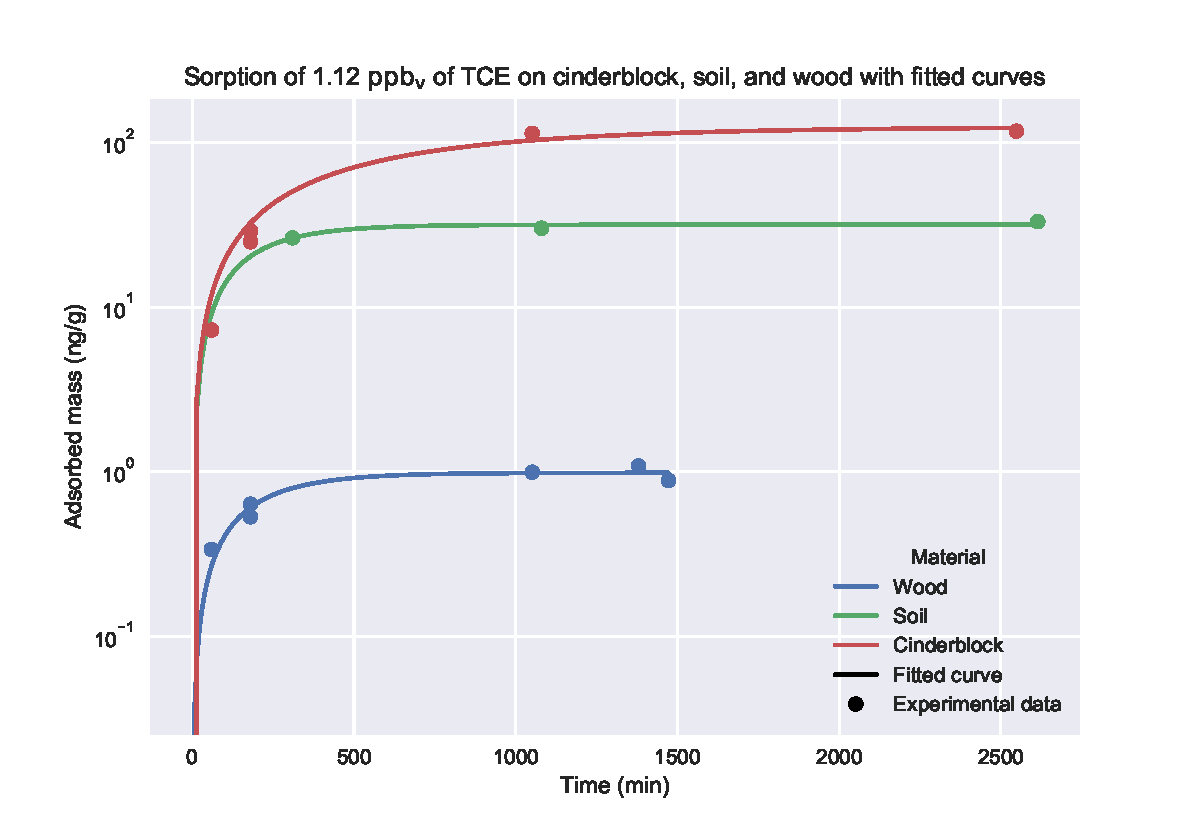
\includegraphics[width=\textwidth]{sorption_fit.pdf}
  \caption{Experimental data of sorption of TCE onto three select materials as well as fitted sorption rates based on the kinetic model \eqref{eq:sorption_rate}.}
  \label{fig:sorption_fit}
\end{figure}

% TODO: Shuai: Some thoughts or comments about these values? I.e. why is cinderblock so much larger?
Table \ref{tbl:sorption_fit} shows the fitted parameters for the tested materials.
Based on this these results we can see that cinderblock and soil have orders of magnitude larger sorption capacities than wood or drywall does.
We can also see by the $k_2$ values that soil and cinderblock sorb quickly, much faster than a material with similar sorptive capacity such as paper.\par
\textit{Note: Here I envision some explanation/discussion on why there is a such a big difference in sorptive capacities. I've asked Shuai to write about this.}

% TODO: Add the relative sorbed mass compared to air. I.e. cinderblock has ~ 7800 more mass for the same volume.
\begin{table}[htb!]
  \caption{Fitted kinetic sorption parameters based on sorption experiment data. Six different types of materials are considered. $k_1$ and $k_2$ are the desorption and sorption constants respectively, and $K$ is the sorption equilibrium constant.}
  \label{tbl:sorption_fit}
  \centering
  \begin{tabular}{l c c c}
    \toprule
    Material & $k_1 \; \mathrm{(1/hr)}$ & $k_2 \; \mathrm{(1/hr)}$ & $K$ \\
    \hline
    Wood & 0.32 & 44.90 & $7.10 \cdot 10^{-3}$ \\
    Drywall & 0.41 & 87.94 & $4.65 \cdot 10^{-3}$ \\
    Carpet & 0.26 & 58.74 & $4.42 \cdot 10^{-3}$ \\
    Paper & 0.04 & 88.37 & $4.55 \cdot 10^{-4}$ \\
    Soil & 0.34 & 2636.57 & $1.30 \cdot 10^{-4}$ \\
    Cinderblock & 0.10 & 4175.16 & $2.40 \cdot 10^{-5}$ \\
    \bottomrule
  \end{tabular}
\end{table}

\subsection{Soil Sorption's Retarding Effect}\label{sec:retardation_effect}

Building pressurization is a key factor in VI that influences the advective contaminant transport.
The magnitude of change in response to a pressurization change is significantly influenced by a range of factors, such as soil permeability, foundation depth, or soil moisture, and of course - sorption, which we will focus on.
To investigate the effect that soil sorption has on contaminant soil mass transport in the VI context, we run two types transient simulation where initially the modeled structure is depressurized at a steady -5 Pa.
At the start of the simulation, the building building is further depressurized to -15 Pa \eqref{eq:equilibrium_depressurization}, or overpressurized to 15 Pa \eqref{eq:equilibrium_overpressurization}, and the simulation is allowed to run for 72 hours. % TODO: Update this once the new simulations are done.
\begin{align}
  \text{Depressurization}: \; \Delta p_\mathrm{in/out} &= \begin{cases}
    -5, \; &t = 0 \; \mathrm{(hr)} \\
    -15, \; &0 < t \leq 72 \; \mathrm{(hr)}
\end{cases}\label{eq:equilibrium_depressurization}\\
\text{Overpressurzation}: \; \Delta p_\mathrm{in/out} &= \begin{cases}
  -5, \; &t = 0 \; \mathrm{(hr)} \\
  15, \; &0 < t \leq 72 \; \mathrm{(hr)}
\end{cases}\label{eq:equilibrium_overpressurization}
\end{align}
For each of these cases, the simulation is run using two different soil types - sand and sandy loam.
Sand is assumed here to not sorb any TCE, while for sandy loam a range of sorption isotherms are used.
These range from no sorption ($K_\mathrm{ads} = 0 \; \mathrm{(m^3/kg)}$) to the experimentally determined sorption isotherm ($K_\mathrm{ads} = 5.28 \; \mathrm{(m^3/kg)}$) in intervals multiplicative by $10^{-2}$. With the experimentally determined isotherm, we see that the ratio between sorbed concentration and soil-gas phase concentration is 7708, i.e. there is a much larger amount of sorbed contaminant.
When $K_\mathrm{ads} = 5.28 \cdot 10^{-4} \; \mathrm{(m^3/kg)}$ this ratio is roughly unity (0.77), which is good to keep in mind in the following discussion. % TODO: Make sure you change this value if you rerun the simulation later with a different H
These ranges of values can be used both to represent a soil that has a smaller sorptive capacity or a situation where the sorbed and gas phase has not quite reached equilibrium.\par

\begin{figure}[!htb]
  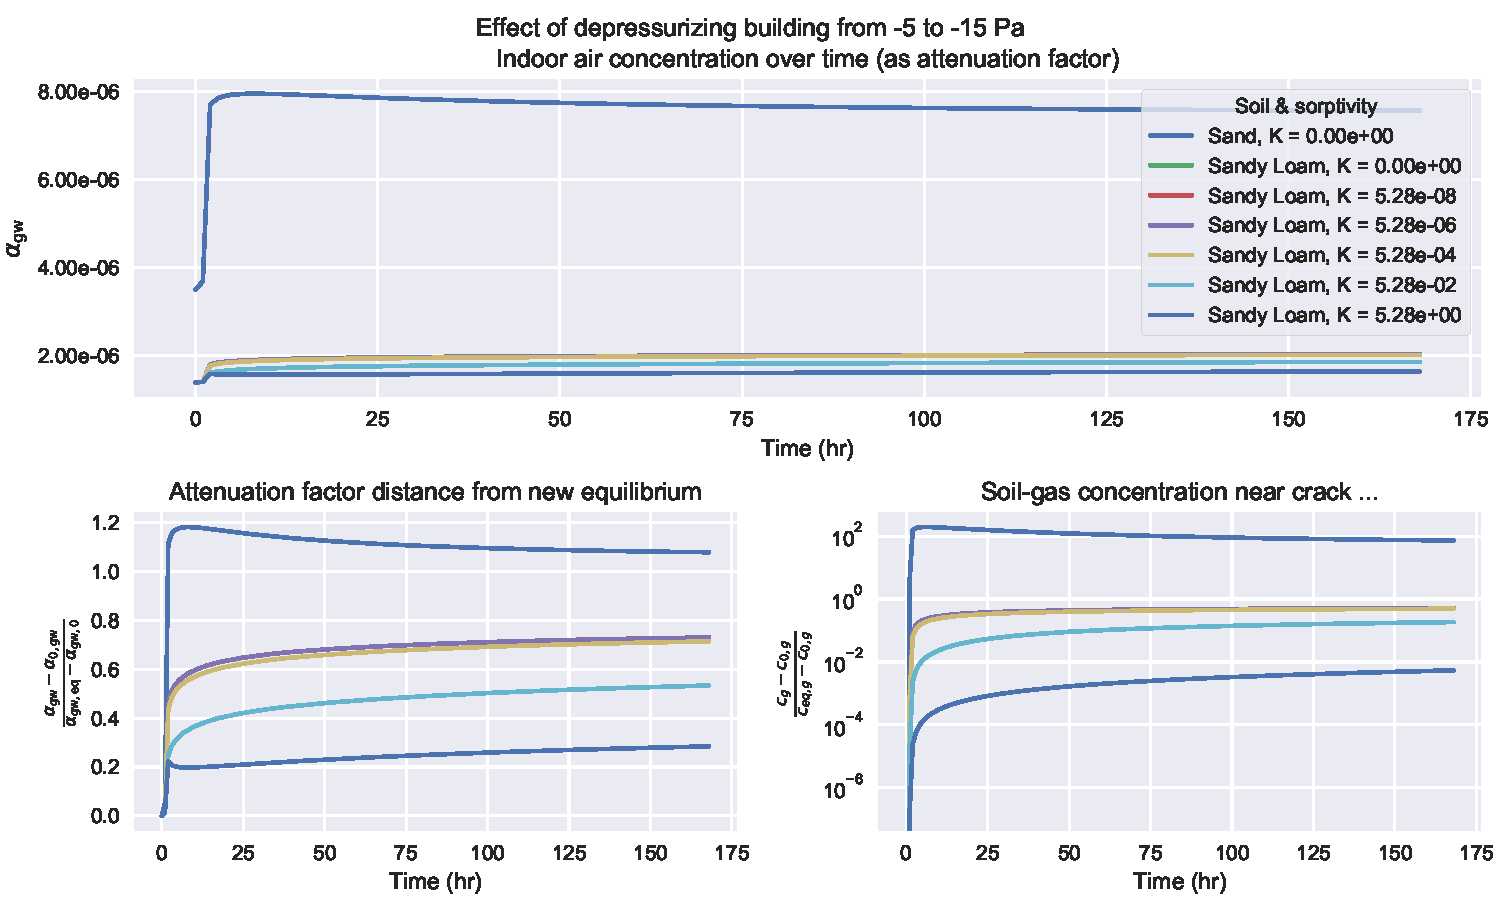
\includegraphics[width=\textwidth]{equilibrium_retardation_depressurization.pdf}
  \caption{}
  \label{fig:equilibrium_depressurization}
\end{figure}

The top panel of Figure \ref{fig:equilibrium_depressurization} shows the indoor air contaminant concentration as the simulated building is undergoing the pressurization in \eqref{eq:equilibrium_depressurization} case.
Here we can see that for the when the surrounding soil consists of sand, the indoor concentration increases rapidly as the building is further pressurized.
The rate of increase decreases significantly for the sandy loam cases, and progressively retards are the sorbed mass increases ($K_\mathrm{ads}$ increases).\par

The bottom left panel shows how far away the indoor air concentration (as attentuation factor) for each case is from reaching equilibrium.
At the start of the simulation, the building starts with an attenuation of $\alpha_0$, which is the steady-state concentration when the building is pressurized with -5 Pa.
As the building is further depressurized to -15 Pa, the indoor air concentration will approach a new equilibrium state $\alpha_{eq}$ (the result of which is from a steady-state simulation at that pressurization).
By plotting $\frac{|\alpha-\alpha_0|}{|\alpha_{eq}-\alpha_0|}$ we can easily see how far away we are from the new equilibrium state, and a value of 0 represents that we are at the initial concentration, i.e. $\alpha = \alpha_0$, and a value of 1 represents $\alpha = \alpha_{eq}$, i.e. that the new equilibrium has been reached.\par

This sort of analysis is applied to the bottom right panel as well, but instead of the indoor air concentration (as attentuation factor), we consider the average soil-gas concentration in a 5 cm diameter cylinder that envelop the entire perimeter crack.
The choice of 5 cm is arbitrary, but helps illustrate what happens in the near-foundation-crack region soil-gas concentration, changes in which allow us to better understand how the contaminant is transported into the building from the soil.
The same could be done for the soil-gas velocity of course, but the rate of soil-gas velocity change is virtually the same for all of these cases, and reaches the new equilibrium velocity very quickly (much faster than the concentration) and is thus omitted from the figure.\par

Before discussing the role of sorption here, we can first compare the non-sorbing sand and sandy loam cases.
Due to the higher permeability and lower moisture content, sand is significantly more permeable to gas flow than sandy loam (see Table \ref{tbl:model} for permeability values).
Consequently the advective transport through the foundation crack is much more significant, which is indicated by a Péclet number of around 4 versus 0.2 at a -15 Pa pressurization for sand and sandy loam respectively.\par

Due to the advection dominated transport mechanism in the sand case, the indoor air concentrations are temporarily elevated above the equilibrium concentration at -15 Pa, while the soil-gas concentration moves further away from equilibrium.
(Note that the absolute distance from equilibrium is plotted in Figure \ref{fig:equilibrium_depressurization} which is why at first glance one might think that the soil-gas concentration is two order of magnitude higher initially, but actually is two order of magnitude lower.)
This phenomena occurs because initially more contaminants are drawn into the building from the near crack area than can be resupplied, temporarily depleting the local soil-gas contaminant concentration.\par

One can notice that many of the sandy loam lines overlap, and start diverging from each other when $K_\mathrm{ads} = 5.28 \cdot 10^{-4} \; \mathrm{(m^3/kg)}$, at the point where the ratio of sorbed and soil-gas concentration are roughly equal.
We see that this divergence occurs simultaneously in the indoor air and soil-gas contaminant concentration.
However, since the indoor air concentration depend on the soil-gas concentration, we know that this is where the relevant difference is.\par

The simple reason for this is that it is at this threshold the sorptive contribution to the retardation factor \eqref{eq:retardation_factor} starts to becomes larger than the other terms.
\begin{equation}
   \rho_b K_H K_\mathrm{ads} > \theta_w + \theta_g K_H
\end{equation}
Thus it is at this point that the contaminant transport in the soil starts to become retarded by sorption.
The physical reason for this is that the partitioning between the various phases gives a residence time as the contaminant is transported.
Under VI conditions, the values of $\theta_w + \theta_g K_H$ are bounded to relatively small values, while $K_\mathrm{ads}$ can vary by orders of magnitude, making sorption potentially a very significant retarder for soil transport.\par

We can also note that the retarding effect of sorption also somewhat depends on the contaminants Henry's Law constant $K_H$, bulk density $\rho_b$ and the moisture content $\theta_w$.
For instance if the ambient temperature is higher, then contaminant $K_H$ is likewise larger, and sorption induced retardation is greater.
Generalizing this is difficult however, as $K_\mathrm{ads}$ is also temperature dependent, and the interplay between these may be complicated.
Nevertheless this hints that there may be a climate/weather component to how significantly sorption induced retardation is.\par

Figure \ref{fig:equilibrium_overpressurization} shows the same sort of analysis as in Figure \ref{fig:equilibrium_depressurization} but with the building pressurization following \eqref{eq:equilibrium_overpressurization}.
The results here are more or less the same, with the notable exception that in the sand case, the final equilibrium concentration is not initially exceeded.
As the building is overpressurized, the indoor contaminant are pushed out into the soil.
Since the indoor air concentration is lower than the soil-gas concentration, this is entirely expected.\par

\begin{figure}[!htb]
  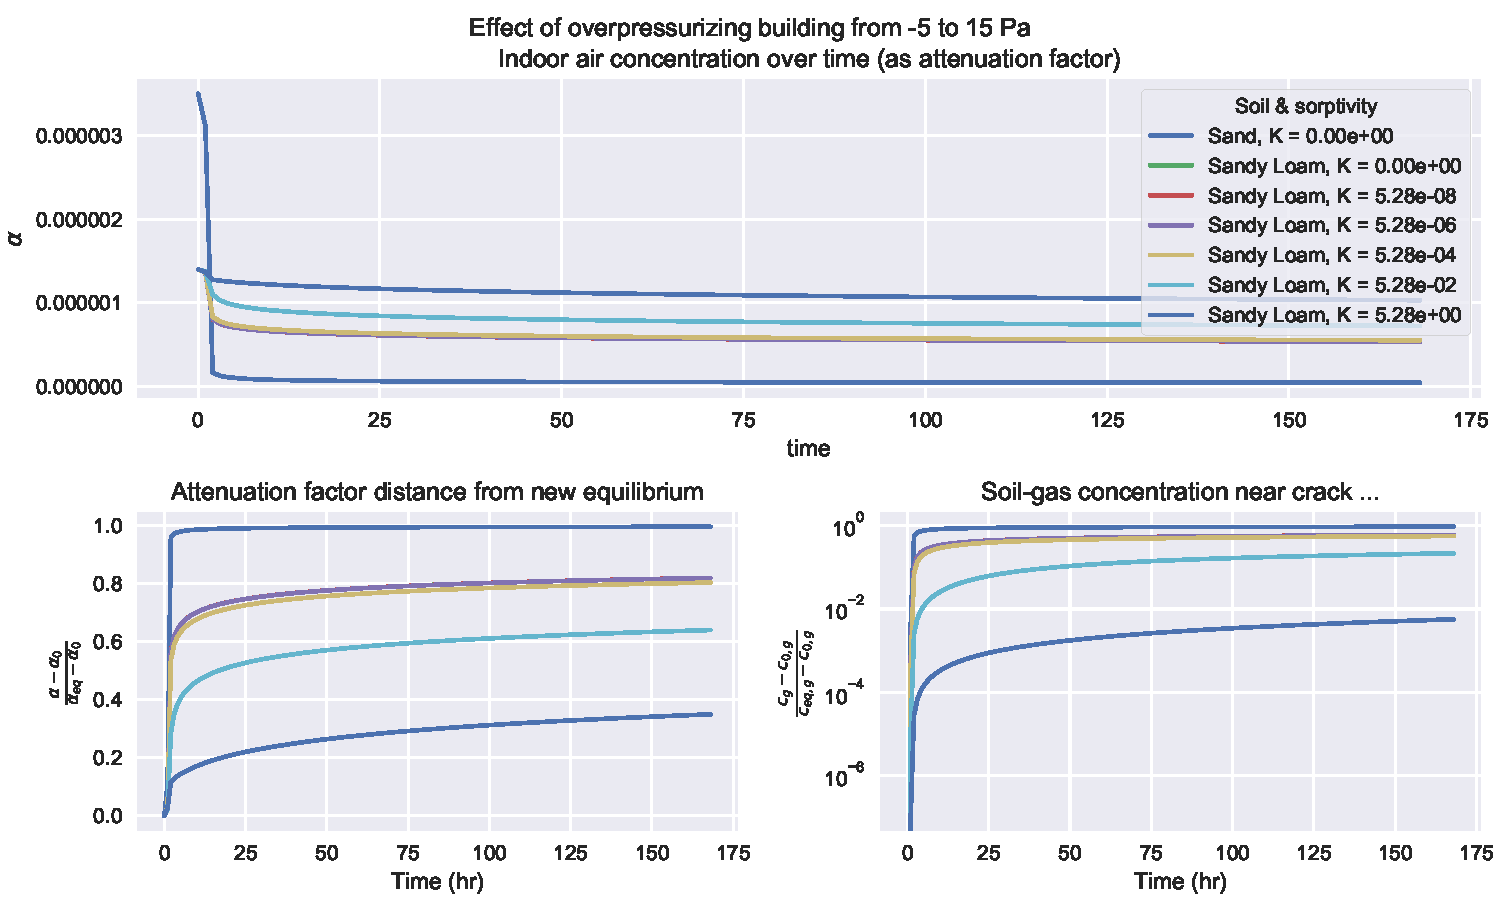
\includegraphics[width=\textwidth]{equilibrium_retardation_overpressurization.pdf}
  \caption{}
  \label{fig:equilibrium_overpressurization}
\end{figure}

% TODO: Some concluding remarks or keep this solely for the conclusion section?

\subsection{Indoor Material Sorption And Dynamics}\label{sec:results_indoor_sorption}

Now we turn to exploring the effect of sorption onto/from various indoor materials has on the indoor air contaminant concentration, again through our model.
For these simulations we assume that there is no soil sorption.
To study this we consider the basement (the indoor air space) and assume that the inside surfaces are entirely made up of one of the materials we studied in \ref{sec:results_sorption_fit}.
We also assume that the material covering the indoor surfaces has a certain thickness or depth that the contaminants can penetrate - giving a certain volume or mass of sorbing material in the indoor.
Table \ref{tbl:sorbed_material} shows the surface area, penetration depth, and volume of each material studied.
While obviously some of these rooms are non-conventional and arbitrarily designed, i.e. you're unlikely to find a room with carpeted walls, floors, and ceiling, they do present some limiting cases of the potential effect of sorption onto/from these materials.\par

% TODO: Do I want to include some more information/data here? Sorbed mass at t0?
\begin{table}[htb!]
  \centering
  \begin{tabular}{l c c}
    \toprule
    Material & $d_\mathrm{p} \; \mathrm{(mm)}$ & $V_\mathrm{mat} \; \mathrm{(m^3)}$ \\
    \hline
    Cinderblock & 5 & 1.6 \\
    Wood & 1 & 0.32 \\
    Drywall & 10 & 3.2 \\
    Carpet & 10 & 3.2 \\
    Paper & 0.1 & 0.032 \\
    \bottomrule
  \end{tabular}
  \caption{The assumed contaminant penetration depth and subsequent volume of the sorbing indoor materials. The material surface area is assumed to be the same, and each material completely cover the surfaces of a 10x10x3 meter room.}
  \label{tbl:sorbed_material}
\end{table}

The modeled building then undergoes a pressurization cycle, where at start of the simulation it is depressurized at -5 Pa and at steady-state.
The building is then sequentially depressurized to -15 Pa, then pressurized to 15 Pa, and finally again depressurized to -5 Pa.
For each sequence, the new pressurization is maintained for 24 hours.
This pressurization cycle may be seen in the top left panel of \ref{fig:indoor_sorption_cycle}.
The choice of pressurization cycle is somewhat arbitrary, but ours can be used to represent limiting cases of natural pressurization variation, or artificially induced pressurization.
Figure \ref{fig:indoor_sorption_cycle} shows the result of these simulations.\par

The change in indoor air contaminant concentration over this pressurization cycle is shown in the bottom panel of Figure \ref{fig:indoor_sorption_cycle}.
First we consider the reference case - where there is no sorbing indoor materials present.
(The blue line is the reference case, which may be difficult to see as the wood and carpet lines overlap.)
Here we see that as the building is depressurized, the indoor air contaminant concentration increases quickly in response to the pressurization change, and is approaching an equilibrium.\par

% TODO: Plot the sorption rate r normalised to the entry rate n_ck? Should be ~1 when materials becomes saturated. Nice way to non-dimensionalize this too. Maybe as second axis plot on the top right panel?
\begin{figure}[!htb]
  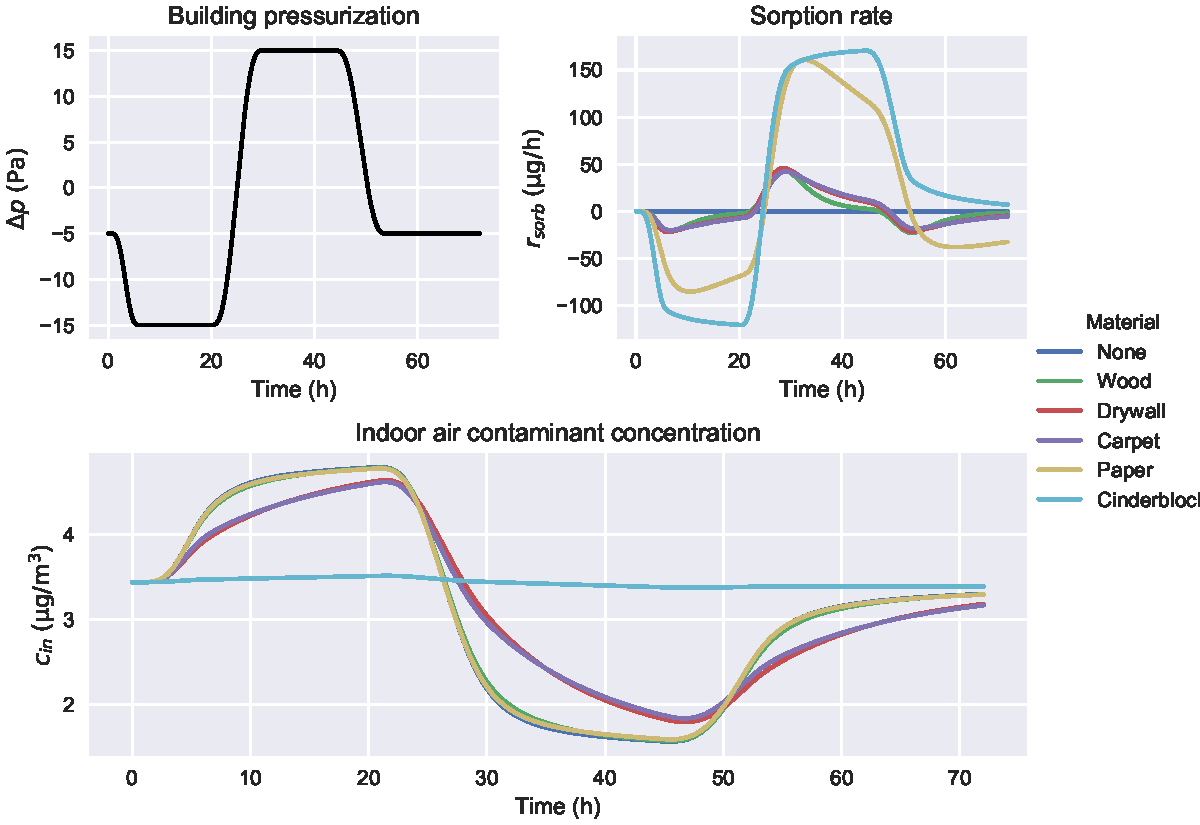
\includegraphics[width=\textwidth]{sorption_indoor_cycle.pdf}
  \caption{
  Comparison of how sorption onto/from various indoor materials affect the indoor air contaminant concentration (bottom) of a building that undergoes a pressurization cycle (top left). The rate of de- and sorption for each considered material during the cycle are also shown (top right) and is governed by \eqref{eq:sorption_rate}. A positive value means that contaminant vapors are being sorbed onto/into the material and a negative means the material is desorbing into the indoor air space.}
  \label{fig:indoor_sorption_cycle}
\end{figure}

By observation we can see that the presence of the various studied building materials in the indoor environment has a very different effect on the change in indoor air contaminant concentration.
The presence of wood and carpet has close to no effect on the indoor air concentration.
While cinderblock has a very significant effect, preventing almost any change in indoor concentration.
Drywall and carpet is in the middle significantly delays the rate of change in the indoor concentration, but for each 24 hour cycle, roughly the same indoor concentration is reached as the reference case.\par

The disparity of these result is explained by the the top right panel of Figure \ref{fig:indoor_sorption_cycle}.
Here the de- and sorption rates in $\mathrm{\mu g/hr}$ for each considered indoor material is shown.
A positive and negative value here indicate that contaminant is desorbed respectively sorbed to and from the material.
To understand this figure, it is useful to refer back to Table \ref{tbl:sorption_fit} which show the sorption and desorption rate constant $k_1$ and $k_2$ respectively, and the sorption equilibrium constant $K$ (a smaller value indicate a larger sorptive capacity).\par

First we consider to the depressurization part of the cycle (1-25 hours).
(Here see that the reference case has no sorption at all, by definition.)
And similar to the indoor concentration panel, we see that the wood, drywall, and carpet cases overlap.
This is explained by these materials have similar sorptive capacities ($K$) and sorptive rates ($k_2$).
Paper by contrast has a similar shape to the three previously mentioned, while the magnitude is significantly larger.
This is because the $K$ value for paper is one order of magnitude larger, indicating that wood, drywall, and carpet saturate with contaminant vapors over the time period, while paper does not.
Cinderblock has a further order of magnitude larger $K$ value, thus is even further away from being saturated, which explains the even faster sorption rate.\par

Next we consider the overpressurzation period (25-49 hours).
Again we see here that wood, drywall, and carpet behave the similarly for the same reasons as before, i.e. the desorption rate constants $k_1$ and sorption equilibrium constants $K$ are similar.
This means that these reach the new sorbed contaminant saturation at roughly the same time.\par

Here it is important to note that due to the diffusion dominated transport through the foundation crack, even though the building is overpressurized, there is substantial contaminant entry.
And because the sole contaminant source is the modeled contaminated groundwater, the sorbed equilibrium is relative to this entry rate.\par

Paper and cinderblock initially behave very similarly during the overpressurization period and desorb contaminants quickly.
However, paper reaches its saturation limit after a relatively short time, while cinderblock has not even at the end of the overpressurization cycle.
Since the desorption rate constants $k_2$ are relatively similar for the materials, thus this disparity is primarily due to the different sorption equilibrium constants $K$.\par

Lastly, we consider the final period where the pressurization goes back to its initial state (49-72 hrs).
Here we see that the reference case does not quite return to the initial indoor concentration.
Thus the contaminant entry rate has not equilibrated yet, due to the soil contaminant concentration has not done so either.
Like in the previous analysis we again see that the wood, drywall, and carpet cases don't differ from the reference.
The paper case is slightly more different, but for the same reasons that have already been discused.
Cinderblock is unique here though, as we clearly see that it is releasing contaminants, due to the previous change in contaminant concentration has been so significantly retarded.\par


From this simulation work we can see how varied the effect of sorbing indoor materials are.
Most of the tested materials only have a moderate effect on the indoor air contaminant concentration dynamics, with the notable exception of cinderblock, which effectively enforces as pseudo-steady-state.
However we also see from the analysis of the sorption dynamics that the de- and sorption rate constants $k_1$ and $k_2$ are less important than the sorptive capacity $K$ of the material.\par

\subsection{Indoor Material Sorption And Mitigation}\label{sec:results_indoor_mitigation}

The work done by us and others have shown the large sorptive capacities of various common materials.
The desorption of the sorbed contaminants may have significant impact on the efficacy of various mitigation systems.
To investigate this we turn to our model and consider a scenario where initially the modeled building is depressurized with -5 Pa and at the start of the simulation some perfect mitigation scheme is  turned on and the contaminant entry $n_\mathrm{entry}$ in \eqref{eq:cstr} goes to zero.
We also assume that for each case, the indoor environment contains the same amount of indoor material as described in section \ref{sec:results_indoor_sorption}.
The air exchange rate is assumed to remain a constant 0.5 per hour for the entire 72 hour simulation time.\par % TODO: Update this time if you run a longer simulation later.

The decrease in indoor air concentration (as attenuation factor $\alpha$) for each simulated case is seen in Figure \ref{fig:sorption_mitigation}.
As excepted, when there is no sorbing indoor materials, i.e. our reference case, the indoor concentration decreases log-linearily.
We can also see that the contaminant desorption from the materials maintain a higher indoor air concentration relative to reference, with cinderblock again shown to have the great impact.\par

\begin{figure}[!htb]
  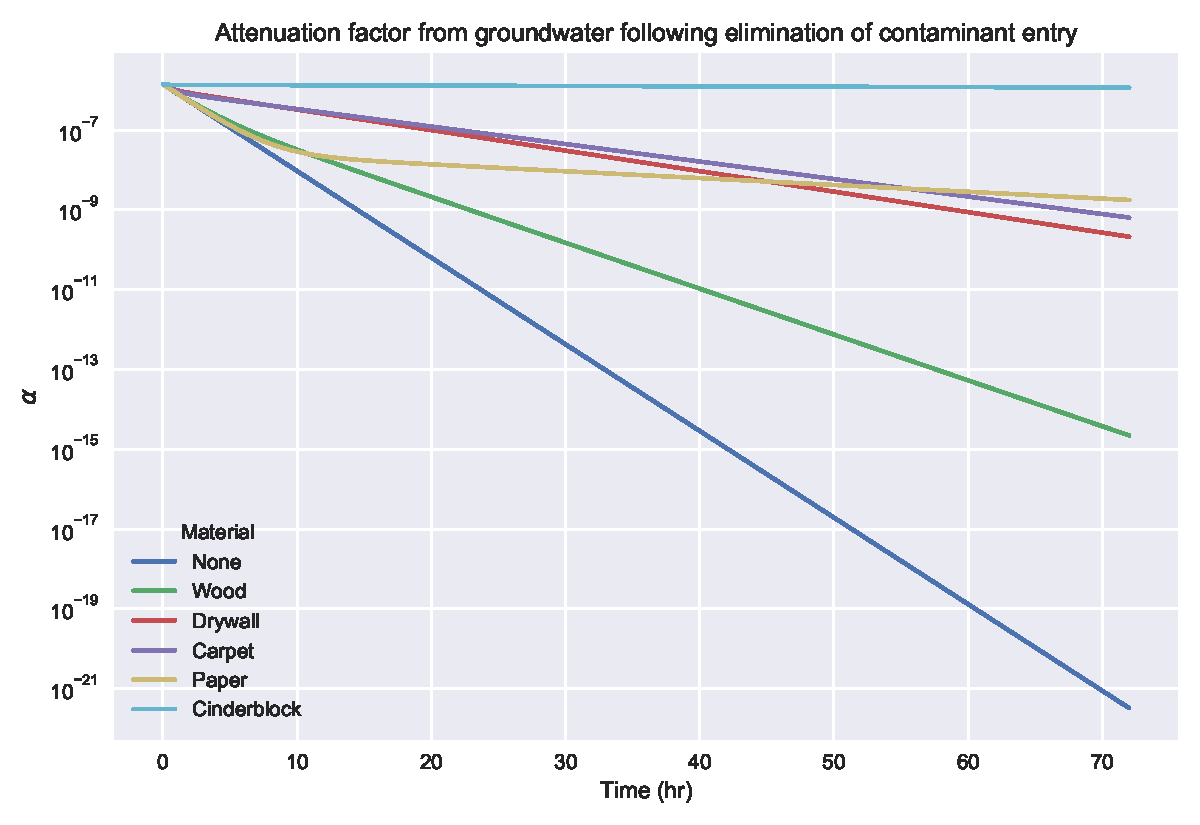
\includegraphics[width=\textwidth]{sorption_mitigation.pdf}
  \caption{}
  \label{fig:sorption_mitigation}
\end{figure}

\textit{Note that this section is still incomplete as I am still working on expanding/improving the analysis/figure.}

\section{Conclusions}\label{sec:conclusions}


\section*{Acknowledgements}
This project was supported by grant ES-201502 from the Strategic Environmental Research and Development Program and Environmental Security Technology Certification Program (SERDP-ESTCP).\par

Declaration of interest: none

\clearpage
\clearpage
\begin{table}[htb!]
  \centering
  \begin{tabular}{l l}
    \toprule
    % A/ALPHA
    $A_\mathrm{ck}$ & Crack area \\
    $A_e$ & Air exchange rate \\
    $\alpha, \; n, \; m, \; l$ & van Genuchten parameters \\
    $\alpha_\mathrm{gw}$ & Attenuation from groundwater contaminant vapor source \\
    % C
    $c_\mathrm{in}$ & Indoor air contaminant concentration \\
    $c_w$ & Soil-water contaminant concentration \\
    $c_g$ & Soil-gas contaminant concentration \\
    $c_s$ & Sorbed contaminant concentration in the soil \\
    $c_\mathrm{sorb}$ & Sorbed contaminant concentration on indoor material \\
    $c_\mathrm{gw}$ & Contaminant groundwater concentration \\
    % D
    $D_\mathrm{eff}$ & Effective diffusion coefficient \\
    $D_\mathrm{air}, \; D_\mathrm{water}$ & Diffusion coefficient in air/water \\
    $d_p$ & Penetration depth of sorbed contaminant in material \\
    % J
    $j_\mathrm{ck}$ & Contaminant molar flux through the foundation crack \\
    % K
    $\kappa$ & Saturated soil permeability \\
    $K_{ads}$ & Sorption partition coefficient in soil \\
    $K$ & Sorption partition coefficient \\
    $K_H$ & Dimensionless Henry's law constant \\
    $k_r$ & Relative permeability \\
    % L
    $L_\mathrm{slab}$ & Thickness of the foundation slab \\
    $\lambda$ & Eigenvalue \\
    % M
    $M$ & Molar mass \\
    $\mu$ & Contaminant vapor viscosity \\
    % N
    $n_\mathrm{ck}$ & Contaminant entry rate through the foundation crack \\
    % P
    $\mathrm{ppb_v}$ & Part-per-billion by volume \\
    $p$ & Pressure in soil \\
    $p_\mathrm{in}$ & Indoor pressure relative to outside \\
    $p_\mathrm{out}$ & Ambient outside pressure \\
    % R
    $\rho$ & Density \\
    $\rho_b$ & Bulk density \\
    $R$ & Retardation factor \\
    $r_\mathrm{sorb}$ & Rate of sorption \\
    % S
    $\mathrm{Se}$ & Soil water saturation \\
    % T
    $\theta_g$ & Vapor/gas filled porosity \\
    $\theta_w$ & Water filled porosity \\
    $\theta_r$ & Residual water filled porosity \\
    $\theta_s$ & Saturated or total porosity \\
    % U
    $\vec{u}$ & Soil-gas velocity (vector quantity) \\
    $u_{ck}$ & Soil-gas velocity through the foundation crack \\
    % V
    $V_\mathrm{bldg}$ & Building/control volume \\
    $V_\mathrm{mat}$ & Volume of sorbing material \\
    $\vec{v}$ & Eigenvector \\
    % Z
    $z$ & Elevation above groundwater \\
    \bottomrule
  \end{tabular}
  \caption{List of abbreviations and nomenclature}\label{tbl:abbreviations}
\end{table}


\bibliographystyle{elsarticle-num}
\bibliography{references}


\begin{comment}
Main point of this paper:

To explore how sorption affects VI transport in soils and indoor environment,
and the effect that sorption has on efficacy of mitigation systems

Outline:

Introduction:
* Why study sorption in VI?
- Many materials (significantly) sorb VI contaminants.
- No previous studies.
- May significantly affect:
-- Mitigation
-- VI investigations

* What are we gonna do to bridge till gap?
- Measure sorptive capacities at relevant concentrations. Why?
-- Isotherms non-linear w.r.t. concentration & few studies at VI relevant conditions.
-- Pick TCE (contaminant of significant concern).
- Apply results in our VI model.
-- Used extensively before
-- In lieu of a study house this will give some insights

* Outline
- Experimental setup
- Numerical model & governing equations
- Results regarding:
-- Soil transport & sorption
-- Indoor environment transport & sorption (specifically how response of c_in w.r.t. pressurization changes).
-- Reduction of mitigation system efficacy




\end{comment}

\end{document}
